\section{Model Generation}
The main goal of the present work, as stated before, is to recreate a three-dimensional virtual model of histological tissue as faithfully as possible and then, to perform a planar sectioning on it to emulate virtually the traditional histological specimen preparation procedure. The creation of a model of such complex structures is definetly an high-level problem, and it has required a carefull designing, made of successive phase of improvements. In this work I will report only two specific attempts of modelization: the first aiming to report pancreatic tissue, and the second oriented toward dermatic tissue.

\subsection{Pancreas Tissue Model} \label{ssec:panc_tis_mod}
The Pancreas is an internal organ of the human body, part of both the digestive system and endocrine system. It acts as a gland with both endocrine and exocrine functions, and it is located in the abdomen behind the stomach. Its main endocrine duty is the regulation of sugar levels in blood and the secretion of hormones, as insulin, glucagon. While, as a part of the digestive system it acts as an exocrine gland secreting pancreatic juice. The majority of pancreatic tissue has a digestive role, and the cells with this role form clusters (\textit{acini}) around the small pancreatic ducts, and are arranged in lobes. The acinus secrete inactive digestive enzymes called zymogens into the small intercalated ducts which they surround, and then in the pancreatic blood vessels system \cite{Pancreas}. In Figure \ref{fig:panc_struct} is reported a picture of pancreas, with its structure and its placement in the human body.

\begin{figure}
    \centering
    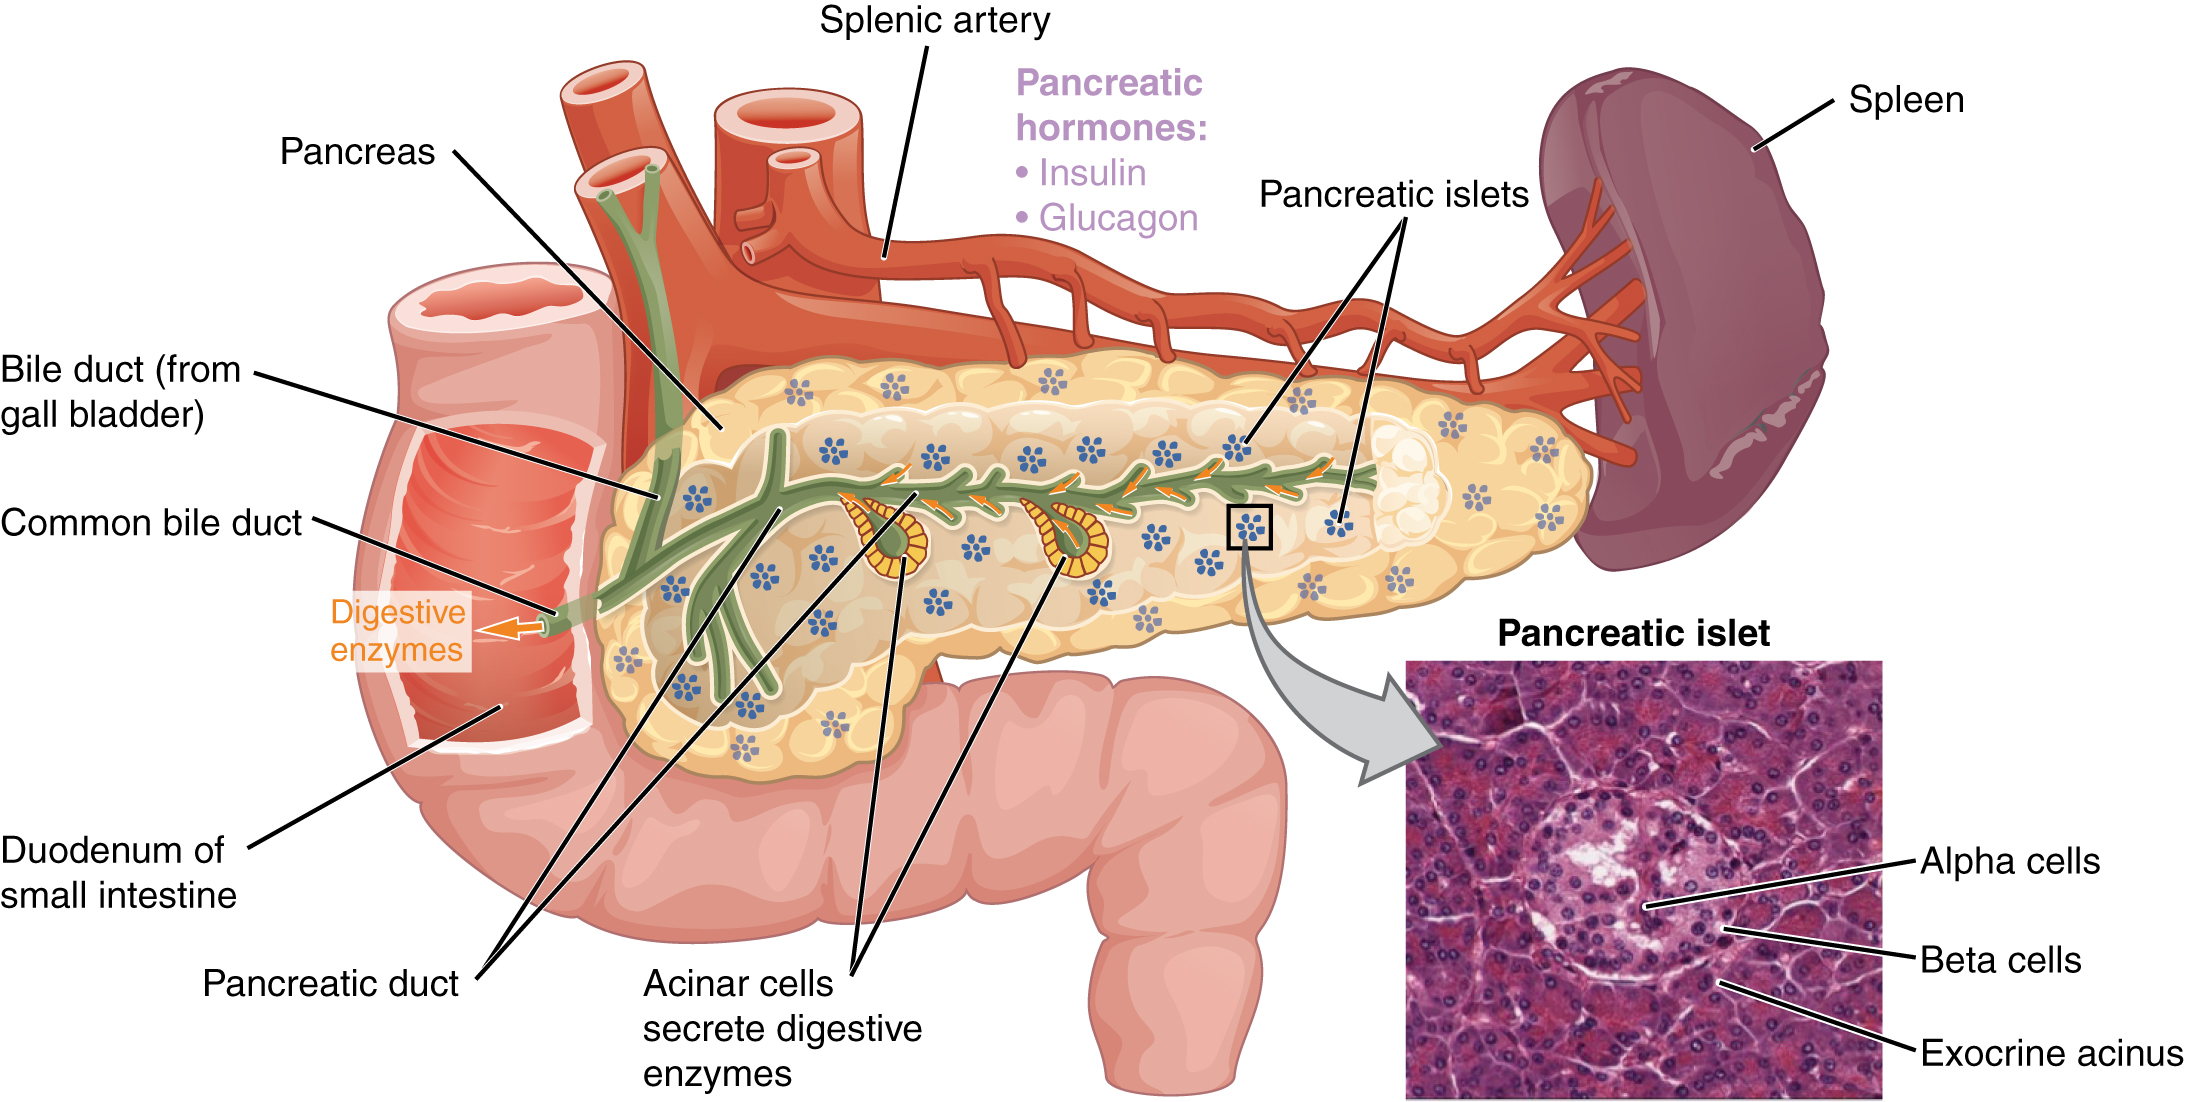
\includegraphics[width = 0.8\textwidth]{images/panc_struct}
    \caption{A picture of pancreas' structure in its phisiologiacl context. In this picture is clearly visible the macroscopic structure and the galndular organization at microscopic level, and how it reflects in the histological sample.}
    \label{fig:panc_struct}
\end{figure}

All the tissue is actually rich of others important elements as the islets of Langerhans, and sporadic connective tissue allover the structure, which are clearly visible in the traditional histological specimens. In this first attempt of modelization from scratch this second layer of complexity has not been already considered, and the main focus was to reflect only the main structural features on the virtual specimen. Given pancreatic tissue's organization the first features I decided to put emphasis on were: 1) The iterative (with a fractal-like behavior) ramification of blood vassels for the irroration of glandular acinus, 2) The space-filling distribution of acinus in the tissue, in fact we expect an homogeneous density in the organ and to not see \textit{holes} at all inside it. In this secton I will describe step by step all the process I followed to create the model of a portion of pancreatic tissue, and all the interesting pitfalls I overcame.

\hl{[Should I make a bullet point list here? or going along with the text's flux?]}

The first step was took in 2 dimensions, and it was the choice of the right \textit{structure} to emulate the ramification of blood vessels in pancreatic tissue. The choice fell on a particular parametric L-system, as the one shown in Figure \ref{fig:bf_ls}, in section \ref{sec:tech_tool}.

progressively less thick
free ands spheres
avoid superposition
progressive noise in angles


\clearpage
